%\subsection{Device Modeling and Design Flow}
\section{Task 1: Design Methodologies for Emerging Memory Technologies}

This proposed task focuses on device modeling and design flow and optimization
methodologies for memory design using emerging memory technologies.
%\textbf{\underline{HL: Need to be modified.}}
%To help the architectural level and system-level design of
%the SRAM-based or DRAM-based cache and memory, various
%modeling tools have been developed during the last decade. For
%example, CACTI~\cite{CACTI:NORM,PRAM:EVANS,PRAM:eCACTI,PRAM:CACTI60} and
%DRAMsim~\cite{DRAMsim} have become widely used in the
%computer architecture community to estimate the speed, power, and
%area parameters of SRAM and DRAM caches and main memory.
%Similarly, to explore new design opportunities that these emerging
%memory technologies can bring to the designers at architecture and
%system levels, it is imperative to have a high-level model
%for caches and memories built with emerging NVMs, such as MRAM/PCRAM.
%The model needs to provide the extraction of all important parameters, including access latency, dynamic access power, leakage power, die area, and I/O bandwidth \emph{etc.}, to facilitate architecture and system-level analysis and to bridge the gap between the abundant research activities at process and device levels and the lack of a high-level cache and memory model for emerging NVMs.






\subsection{Task 1.1: Device Modeling for Emerging Memory Technology}
The emerging NVM technologies have introduced many new materials, i.e. phase change material Ge$_2$--Sb$_2$--Te$_5$ in PCRAM and magnetic tunneling junction (MTJ) in MRAM. Due to the lack of knowledge on physical mechanisms behind, most of researches on circuit, architecture and system levels nowadays are based on highly-simplified characteristics of the emerging devices. This methodology can cause a large design overhead, increase the production cost, and reduce the design margin, especially in the highly scaled technology with large process variations. For example, our previous work~\cite{Chen08} showed that after adopting a dynamic MTJ model that can take into account the time-varying electrical inputs in MRAM design flow, the design pessimism can be dramatically minimized and the memory array area can be reduced by more than 40\%. Therefore, one of the important tasks of our proposal is to build device models of emerging NVM technologies. Both dedicated device model and simplified behavioral model will be developed to adapt the requirements at different levels.

Not like SRAM which is based on traditional CMOS technology, new materials are introduced in the emerging NVM technologies. For example, MRAM arises from magnetic tunneling junction (MTJ), and PCRAM technology is based on Ge$_2$--Sb$_2$--Te$_5$.
Due to the lack of knowledge on material physics of these NVM devices, most of research works on circuit, architecture and system levels nowadays are based on highly-simplified characteristics of the emerging devices. This methodology can cause a large design overhead, increase the production cost, and reduce the design margin, especially in the highly scaled technology with large process variations.  For example, the data storage element MTJ at a certain resistance state is usually modeled as a constant resistor by ignoring the dependency of the MTJ resistance on the magnitude of the read/write current driven by the NMOS selection transistor in an MRAM cell. Our previous work~\cite{Chen08} showed that after adopting a dynamic MTJ model that can take into account the time-varying electrical inputs in MRAM design flow, the design pessimism can be dramatically minimized and the memory array area can be reduced by more than 40\%. Therefore, one of the important tasks of our proposal is to build device models of the emerging NVM technologies for circuit design. Both dedicated device model and simplified behavioral model will be developed.
Due to the lack of knowledge on material physics of these NVM devices, most of research works on circuit, architecture and system levels nowadays are based on highly-simplified characteristics of the emerging devices. This methodology can cause a large design overhead, increase the production cost, and reduce the design margin, especially in the highly scaled technology with large process variations.  For example, the data storage element MTJ at a certain resistance state is usually modeled as a constant resistor by ignoring the dependency of the MTJ resistance on the magnitude of the read/write current driven by the NMOS selection transistor in an MRAM cell. Our previous work~\cite{Chen08} showed that after adopting a dynamic MTJ model that can take into account the time-varying electrical inputs in MRAM design flow, the design pessimism can be dramatically minimized and the memory array area can be reduced by more than 40\%. Therefore, one of the important tasks of our proposal is to build device models of the emerging NVM technologies for circuit design. Both dedicated device model and simplified behavioral model will be developed.
The dedicated device models, which will be based on physical mechanisms and corroborated by device measurements, need to satisfy three criteria: (1) both static characteristics (i.e., I-V relationship and high/low resistances) and the dynamic behaviors need be considered; (2) the device parameter fluctuations induced by process variations, such as line-edge roughnesses, oxide thickness fluctuations, and random discrete dopants, will be analyzed; and (3) the models should provide enough accuracy with reasonable runtime. To be compatible to commercial EDA tools, i.e., HSPICE from Synopsys~\cite{synopsys} and Spectre from Cadence~\cite{cadence}, Verilog-A or C language will be utilized to implement these models. The dedicated model will be used for memory array optimization and timing/power analysis.

\begin{wrapfigure}{r}{0.45\textwidth}
\centering
\centering
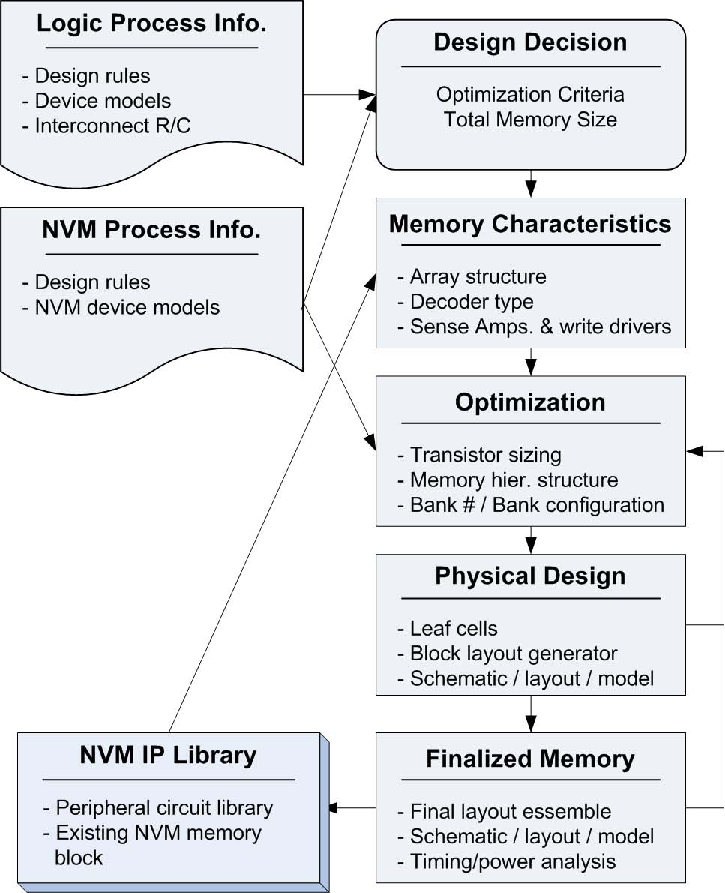
\includegraphics[width=0.45\textwidth]{./figure/3_flow.pdf}
\caption{The proposed design methodology for the emerging NVMs.}
\label{flow}
\vspace{-20pt}
\end{wrapfigure}

On top of the dedicated device model, critical timing and function related parameters, i.e. read/write access time and critical switching current, will be extracted and fed into the simplified behavior models. High-level languages, i.e. VHDL/Verilog or C will be used. The simplified conceptual model is expected to provide sufficient accuracy and %for logic and functionality analysis.
can be easily integrated in the commercial EDA tools and design methodologies such as \emph{Primetime} and \emph{Timemill} from Synopsys~\cite{synopsys} for more thoroughly analysis, \emph{i.e.}, the critical path timing at design corners.

\subsection{Task 1.2: Memory Circuit Design Flow}

Another important task of our proposal is to build a design environment that can be seamlessly integrated the emerging NVMs with the existing CMOS logic design flow. Our goal is to use generic memory cells to generate the memory specified by the user. The basic generation methodology and flow is illustrated in Figure~\ref{flow}.
\begin{wrapfigure}{r}{0.55\textwidth}\centering \centering   \includegraphics[width=0.55\textwidth]{./figure/HL-flow.pdf}
\caption{The proposed scope of device modeling and circuit analysis methodology for the emerging NVMs.}\label{flow}  \vspace{-20pt}
\end{wrapfigure}

The flow will start working technology specification. Note that the NVM technology could be completely separated from logic process. A high level NVM device model could be used to make initial design decision. The next step is to define the specific characteristics of the desired memory. These characteristics include memory size, array structure, sensing scheme, decoders, etc. Some circuitries can be imported from NVM IP (Intelligence Properties) library to reduce design cycle. Moreover, the constraints for the given application, if any (i.e. energy, delay, area, and noise margin), need to be defined in this stage. Optimization is the key step within the whole design flow so that he dedicated NVM device model have to be used. It could take several iterations in order to meet the design specifications. The last two steps deal with the actual memory generation. The design will be checked at the end of each step. Re-optimization may be necessary if the specification could not be satisfied. 

An IP library for emerging NVM technologies will be built with the aid of the proposed design flow. The library will provide a completed set of IP's, including single non-volatile memory cell, peripheral circuit design, and even the whole NMV design based on general design specifications. Those IP's will be used in the researches at architectural and system levels.

The whole methodology and the corresponding outcomes, including device models, memory design flow, and IP's, will be distributed to the architecture and system design community. Our project will build a channel and provide a friendly interface among material development, device fabrication and architecture design.

%=========================================================================
%=========================================================================
\subsection{Task 1.3: Energy/Performance/Reliability Design Space Exploration}

The physical characters of a NVM cell is mainly depends
on the material characters and fabrication process. However, the circuit design
of the memory array, such as the access device of the memory cell, the operational
voltage, and the pheriphral circuitry, can also impact the operation
conditions of the cell, such as current and power consumption. In this task, we propose to explore the design space of the NVM memory array, and study the energy/performance/reliability tradeoffs for memory design with such emerging
memory technologies.

Due to the intrinsic non-volatile characteristics of these emerging memory technology, naturally the read and write behaviors are asymmetric in terms of performance and energy. For example, the write-operation of PCRAM/MRAM requires a large current to be applied for a period of time so that the state of the storage junction is flipped; while the read-operation is realized by applying a small voltage to the cell and sensing the current across the cell.
We propose to analyze the constrained conditions of he design of NVM memory array, and study the sizing of the transistors as well as the operational voltages to investigate the tradeoff of the distinguishability~\footnote{During the read operation, the ratio of high resistance to low resistance in the storage junction reflects the distinguishability between logic 1 and 0}, energy consumption, lifetime and speed. For example, both the width of NMOS access device and word-line
voltage can obviously affect the distinguishability. A higher word-line voltage or a larger NMOS device is more desirable to obtain a high distinguishability. However, the power consumption issues and area consideration always require a low voltage and small device size.
Another example is on the lifetime/energy/performance tradeoff.
For example, the lifetime of PCRAM is represented by the cycling
endurance, which is a function of pulse energy applied for
the memory cell during the RESET writing. The reason for
higher energy pulse induced cycle lifetime degradation
is that the RESET resistance can be saturated when the
writing current is higher than a critical level. This
"over programming`` phenomena can result in lager amorphous
volume, and then degrade the PCRAM��s lifetime. Consequently,
a large write current can help improve the performance, but affect both lifetime and energy. Consequently, depending on the application,
we plan to investigate two optimization strategies: (1) \textit{Energy-driven optimization.} For low power application, such as mobile computing platform, energy consumption may be the most important design goals. We can optimize the word-line and bit-line voltage as well as the transistor sizing of the access NMOS device for memory array to achieve minimal energy consumption while satisfy constrains on lifetime, performance, and area. (2) \textit{Performance-driven optimization.} For high performance application, We can perform the optimization to achieve the best read/write performance while satisfy constrains on lifetime, energy, and area. Such optimization strategies can also be extended to lifetime-driven optimization and density-driven optimization.


\subsection{Preliminary Result and Collaborations:}
The PI Li has built a combined magnetic and circuit design analysis and optimization methodology for MRAM, which has been proved to improve design efficiency significantly~\cite{Chen08} by test-chip design and fabrication at Seagate. We are also one of the first researchers to propose spintronic memristor structures~\cite{Wang09}, which was interviewed by IEEE Spectrum~\cite{Spectrum09}. The corresponding compact model and corner analysis~\cite{Chen09} have also been developed. In this project, we will further extend this methodology to other emerging NVMs, such as PCRAM.

The PSU PI Xie has developed a stacked SRAM cache simulator called 3DCacti~\cite{xie:iccd05-3d, XIE:TVLSI2008-3DCacti}, which has been widely downloaded and used by other researchers. The PI and co-PI have collaborated together when the PI Li was in Seagate, to develop a preliminary version of MRAM simulator for cache stacking~\cite{Xie:dac08,XIE:HPCA09}. Xie also collaborated with Dr. Norm Jouppi from HP Labs, developed a preliminary version of PCRAM simulator~\cite{xie:pcramsim}. We will extend our existing toolsets to support architectural exploration.


